\documentclass{article}
\usepackage[UTF8]{ctex}
\usepackage{geometry}
\usepackage{natbib}
\geometry{left=3.18cm,right=3.18cm,top=2.54cm,bottom=2.54cm}
\usepackage{graphicx}
\pagestyle{plain}	
\usepackage{setspace}
\usepackage{float}
\usepackage{url}
\usepackage{caption2}
\usepackage{graphicx}
\usepackage{datetime} %日期
\renewcommand{\today}{\number\year 年 \number\month 月 \number\day 日}
\renewcommand{\captionlabelfont}{\small}
\renewcommand{\captionfont}{\small}
\begin{document}

\begin{figure}
    \centering
    
\includegraphics[width=8cm]{upc.png}

    \label{figupc}
\end{figure}

	\begin{center}
		\quad \\
		\quad \\
		\heiti \fontsize{45}{17} \quad \quad \quad 
		\vskip 1.5cm
		\heiti \zihao{2} 《计算科学导论》课程总结报告
	\end{center}
	\vskip 2.0cm
		
	\begin{quotation}
% 	\begin{center}
		\doublespacing
		
        \zihao{4}\par\setlength\parindent{7em}
		\quad 

		学生姓名:\underline{\qquad  王春祥 \qquad \qquad}

		学\hspace{0.61cm} 号:\underline{\qquad 1906050123 \qquad}
		
		专业班级:\underline{\qquad 计算1903班 \qquad  }
		
        学\hspace{0.61cm} 院:\underline{计算机科学与技术学院}
% 	\end{center}
		\vskip 2cm
		\centering
		\begin{table}[h]
            \centering 
            \zihao{4}
            \begin{tabular}{|c|c|c|c|c|c|c|}
            % 这里的rl 与表格对应可以看到,姓名是r,右对齐的;学号是l,左对齐的;若想居中,使用c关键字。
                \hline
                课程认识 & 问题思 考 & 格式规范  & IT工具  & Latex附加  & 总分 & 评阅教师 \\
                30\% & 30\% & 20\% & 20\% & 10\% &  &  \\
                \hline
                 & & & & & &\\
                & & & & & &\\
                \hline
            \end{tabular}
        \end{table}
		\vskip 2cm
		\today
	\end{quotation}

\thispagestyle{empty}
\newpage
\setcounter{page}{1}
% 在这之前是封面,在这之后是正文
\section{引言}
计算科学导论,顾名思义,是一个对计算机专业的概括性、引导性的课程。原本是计算机专业大一时应当学习的课程,但是个人是后期通过转专业来到计算机这个专业并且大二上学期课程冲突,所以只得推迟到大三.上学期才来学习这门课程。虽然我现在已经是大三的一名学生,大学的课程学习已经过半,但是通过计算科学导论这门课程我还是学到了许多,下 面我就从课上所学的知识和收获来做一下总结。

\section{对计算科学导论这门课程的认识、体会}
作为一个大二才从储运与建筑工程学院转到计算机科学与技术学院的大三学生,正是因为大一没有学过这门计科导论课程,导致我对计算机这个专业缺乏系统性的认知,导致前两年一直为了凑齐学分而去选课,对于培养方案中的四个选课方向认识不到位。但是经过学习计算科学导论之后,让我对计算机这个专业学习方向和目标有了一个较为深入的认知,每一门课都有其存在的价值与意义,都是为了解决计算科学中的某一特定问题而去开设的。另外作为一名大三的学生,经过前两年的学习,也对计算机专业学习有了一定的基础,再来学习计算科学导论这门课程时有一种温故知新的感觉,正如孙老师上课所说的,计算科学导论这本书可以当成一本故事书来读。在不同的阶段读这本书,会有不同的感觉。
\par

在整个计算科学导论的学习过程中,让我印象最深刻的是方法论的学习。一个学科如果没有问题需要解决,这个学科的生命就结束了,纵观整个科技发展史,可以发现正是问题的提出与解决推动了科学的发展,从丢番图到费马大定理,从$\sqrt{2}$引发的第一次数学危机到希尔伯特提出的二十三个为问题,正是这些问题推动了科学的发展,同样对于计算机科学与技术这个学科而言,同样有三个问题推动了计算机学科的持续发展,这三个问题分别为计算的平台与环境问题、计算过程的能行操作与效率问题和计算的正确性问题,围绕着这三个问题形成了若干主流方向,构成了计算机学科发展的主线。
\par

有了问题便需要解决,而解决问题则需要一个科学的指导,这个指导便是科学哲学的思想方法,科学哲学的思想方法处理问题的步骤可分为三个部分,一个科学的认识、一套科学的方法、一套科学的程序。要解决一个问题,首先要对问题的本质、特点和发展变化规律有一个深入的认知,其次是在科学的认知上通过寻找、建立、改进或者引用,发展解决问题的一套科学的方法,最后在提出科学的解决方法基础上,着眼于解决问题的具体步骤,制定实际解决问题的一个严密的、科学的程序,确定每一步需要做的事情和遇到问题后的处理方案。举一个例子,如何培养创新人才,首先分析一下什么是创新人才,创新型人才是指具有创新精神和创新能力的、在其所在行业的领军人士,由于目前我们主要实行的还是应试型教育,这导致了我们目前培养出的人才缺乏创新意识,所以问题的关键在于目前应试教育阻碍了学生创新意识的形成与发展;其次分析一下如何解决这一问题,培养创新型人才的关键在于打破应试教育,而与应试教育相对的是素质教育,所以我们应当推行素质教育,培养创新型人才;最后提出问题解决的具体方案,推行素质教育,对于学校而言,应当改变固有的教学评估手段,打破唯分论,推行开放性考试,对于学生而言,应当学会举一反三,提高自我创新意识,对于社会而言,应当减少攀比,不能只单单看重学生的分数,而应当支持学生全方位发展,挖掘学生的兴趣,同时支持学校相关工作,共同推动素质教育发展,培养创新型人才。
\par

总之,我认为计算科学导论这门课程主要教会了我一些关于学习计算机科学与技术这么专业的方法论和整体知识框架,在今后的学习生活中我会利用这些方法论去学习更多的专业知识,同时参照计算机科学与技术这门专业的知识框架完善个人知识框架。

\subsection{中国“芯”}

\subsubsection{引言}
近些年来,美国不断对中兴和华为等中国公司进行打压,企图阻止中国芯片研究和制造产业的发展,随之而来的是中兴示弱,华为迎接一轮又一轮的打压并成功活了下来,现在几乎人人都知道中国缺少芯片但是又几乎没有人知道中国目前芯片研发水平,在这里我想调研一下目前中国芯片的发展情况以及我们的缺点所在和相应的对策。
\par

\subsubsection{中国芯片发展现状}
芯片产业主要由三个部分组成,分别为设计、制造、封装测试及装备制造,国芯片产业已经形成包括设计、制造以及封装测试及相关配套完备产业体系。目前,三大产业比例约为3.5∶
2.5∶4,接近于全球芯片产业的3∶4∶3。\citep{xinpian}下面我从芯片产业这三个组成部分分别来说明中国芯片发展现状。
\par

首先是芯片设计,在芯片设计方面,我国有海思、展讯、中兴等龙头企业,并且在2019年
9月6日,华为在德国柏林和北京同时发布最新一代旗舰芯片麒麟990系列,其性能较之前几代有较大的提升。尽管我们在芯片设计方面有着比较大的成就,但是在一些关键技术依然受制于人,第一个便是IP核,我们的芯片设计大多建立在外国公司的IP核基础上,这里的IP全称为Intellectual property,中文翻译为知识产权核,目前麒麟系列芯片采用的是ARM授权的IP核,可以想象如果美国限制我国使用IP核会对我们的芯片设计造成多大的影响;其次便是EDA设计软件,EDA设计软件全称为electronic design automation,中文翻译为电子设计自动化,这是一种芯片设计软件,目前被 Synopsys、Cadence和 Mentor Graphics这三家公司所垄断,并且目前美国已经禁止华为使用EDA软件,试图阻碍我们在芯片设计的发展,但是目前华为海思等公司已经开始自主研发EDA设计软件。
\begin{figure}[H]
\centering
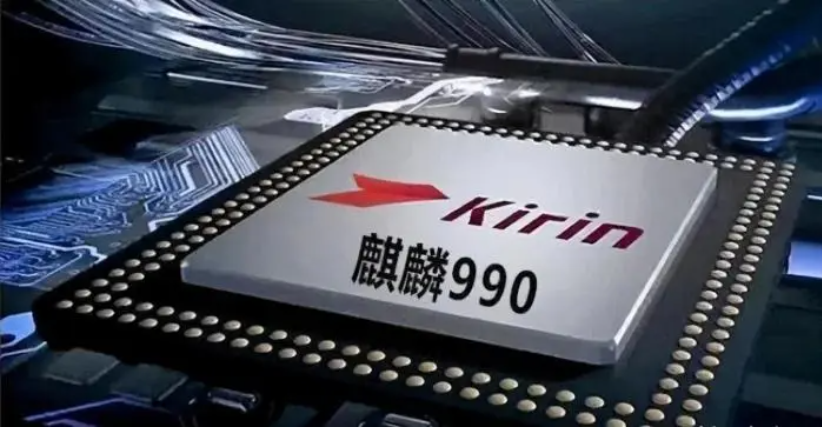
\includegraphics[width=0.7\textwidth]{kirin.png}
\caption{麒麟990芯片}
\label{fig:kirin}
\end{figure}
\par

其次是芯片的制造,目前刻蚀、薄膜、氧化、光刻等一般芯片设备已替代了国外同类产品,成功进入中芯国际等企业的生产线,同时实力最强的中芯国际与华力微电子的工艺水平可以达到 28 nm 与14 nm,但是我们芯片制造的能力与国外还有一定的差距,台积电、三星、英特尔等主流芯片制造商,开始向7 nm 线宽工艺突破,7 nm 工艺成为全球一线芯片制造商发力的焦点。\citep{xinpian2}
\par

最后是芯片的封装测试及装备制造,在芯片封装测试方面,近几年来上游晶圆厂扩建带来了发展空间和下游物联网、智能终端、汽车电子等产品市场的旺盛需求,实现了快速平稳增长。但是在装备制造方面,我们都知道芯片制造当中一个重要的仪器便是光刻机,这是一个制造非常困难的仪器,需要多个国家联合制作才能完成,目前中国已经投入研发,预计不久后将会有国产28 nm的光刻机投入生产使用。除光刻机之外,还有其他一些高科技设备,例如单晶炉、切割机等,目前中国已经能够基本掌握上述设备的生产,并且能够量产12寸和8寸的晶圆。
\par

以上就是国内关于芯片研发与制造的现状,目前国内芯片产品需求量大,据世界半导体行业协会统计,2000-2014年,中国市场规模实现跨越式增长,市场份额位居全球第一,高达50.7\%。这表明,中国的芯片市场已逐渐成为全球芯片不可或缺的力量。目前,在全球的笔记本、平板电脑、智能手机等设备中,高达60\%芯片产自中国。尽管市场规模持续扩大,国产芯片产值增加,但我国芯片自给能力较差,核心产品严重依赖进口,中国企业产品权重仅占10\%,90\%以上的份额为国外产品所圈占。所以中国芯片发展可谓任重而道远。
\par

% \subsubsection{中国芯片未来发展方向}
% 目前促进中国芯片发展有三条路径,一是走国家支持的国产替代路径,二是市场支撑的产品迭代路径,三是突破瓶颈的超越发展路径

% 图片插入的样例:\par
% \begin{figure}[h!]
% \centering
% 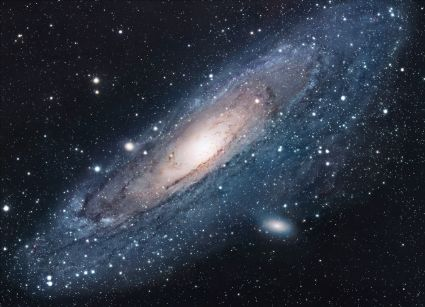
\includegraphics[scale=1.7]{universe}
% \caption{The Universe}
% \label{fig:universe}
% \end{figure}

% \subsection{第二个子标题}
% 表格插入样例:\par

% \begin{table}[h]
%     \centering
%     \caption{这是科学系的花名册}
% \begin{tabular}{rl}
% % 这里的rl 与表格对应可以看到,姓名是r,右对齐的;学号是l,左对齐的;若想居中,使用c关键字。
%     \hline
%     姓名 & 学号 \\
%     \hline
%     张三 & 190704xxxx+++ \\ 
%     李四 & 190704yyyy \\
%     王二五 & 190704zzzz\\
%     \hline
% \end{tabular}
%     \label{table1}
% \end{table}
% \subsection{第三个子标题}
% 这里是引用的样例:\par
% {\bf 注意,仅仅是引用的样例}\par
% 我阅读了图书《机器学习实战》\citep{Harrington2013},引发了我对卷积神经网络的兴趣,于是阅读了期刊论文《卷积神经网络研究综述》\citep{zhoufeiyan},基于对卷积神经网络的深刻认识,我又学习了2018年计算机视觉领域的会议ECCV的会议论文《TextSnake》\citep{long2018textsnake},来探索深度学习落实在生活生产领域的实际意义。\par

\section{进一步的思考}
我们组选的题目是对Docker的探究与分析,我们通过查询相关资料和文献后对Docker有了一个初步的了解,但是其中有许多不完善的地方,经过老师指正后,现将补充后的演讲课题做以下报告。
\subsection{Docker和虚拟机的对比}
\begin{figure}[H]
    \centering
    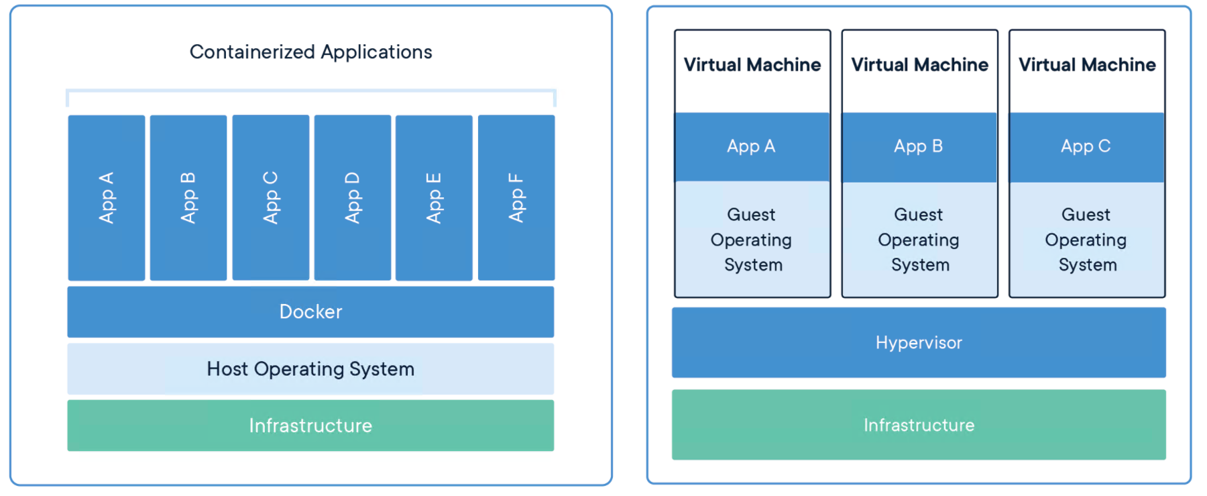
\includegraphics[width=0.95\textwidth]{docker&VM.png}
    \caption{docker和虚拟机的对比}
    \label{fig:docker&VM}
    \end{figure}
比较两图的差异,右图虚拟机的Guest Operating System层和Hypervisor层在docker中被
Docker层和Host Operating System所替代。虚拟机的Guest Operating System即为虚拟机安装的操作系统,它是一个完整操作系统内核;虚拟机的Hypervisor层可以简单理解为一个硬件虚拟化平台,其作用为将底层硬件虚拟化并对上层的虚拟机提供硬件支持。虚拟机实现资源隔离的方法是利用独立的OS,并利用Hypervisor虚拟化CPU、内存、IO设备等实现的。例如,为了虚拟CPU,Hypervisor会为每个虚拟的CPU创建一个数据结构,模拟CPU的全部寄存器的值,在适当的时候跟踪并修改这些值。需要指出的是在大多数情况下,虚拟机软件代码是直接跑在硬件上的,而不需要Hypervisor介入。只有在一些权限高的请求下,Guest OS需要运行内核态修改CPU的寄存器数据,Hypervisor会介入,修改并维护虚拟的CPU状态。
\par

Hypervisor虚拟化内存的方法是创建一个shadow page table。正常的情况下,一个page table可以用来实现从虚拟内存到物理内存的翻译。在虚拟化的情况下,由于所谓的物理内存仍然是虚拟的,因此shadow page table就要做到:虚拟内存-虚拟的物理内存-真正的物理内存。
对于IO设备虚拟化,当Hypervisor接到page fault,并发现实际上虚拟的物理内存地址对应的是一个I/O设备,Hypervisor就用软件模拟这个设备的工作情况,并返回。比如当CPU想要写磁盘时,Hypervisor就把相应的数据写到一个host OS的文件上,这个文件实际上就模拟了虚拟的磁盘。
\par

对比虚拟机实现资源和环境隔离的方案,docker就显得简练很多。docker Engine可以简单看成对Linux的NameSpace、Cgroup、镜像管理文件系统操作的封装。docker并没有和虚拟机一样利用一个完全独立的Guest OS实现环境隔离,它利用的是目前Linux内核本身支持的容器方式实现资源和环境隔离。简单的说,docker利用namespace实现系统环境的隔离;利用Cgroup实现资源限制;利用镜像实现根目录环境的隔离。
通过docker和虚拟机实现原理的比较,我们大致可以得出一些结论:
\par

(1)docker有着比虚拟机更少的抽象层。由于docker不需要Hypervisor实现硬件资源虚拟化,运行在docker容器上的程序直接使用的都是实际物理机的硬件资源。因此在CPU、内存利用率上docker将会在效率上有优势。在IO设备虚拟化上,docker的镜像管理有多种方案,比如利用Aufs文件系统或者Device Mapper实现docker的文件管理,各种实现方案的效率略有不同。
\par

(2)docker利用的是宿主机的内核,而不需要Guest OS。因此,当新建一个容器时,docker不需要和虚拟机一样重新加载一个操作系统内核。我们知道,引导、加载操作系统内核是一个比较费时费资源的过程,当新建一个虚拟机时,虚拟机软件需要加载Guest OS,这个新建过程是分钟级别的。而docker由于直接利用宿主机的操作系统,则省略了这个过程,因此新建一个docker容器只需要几秒钟。另外,现代操作系统是复杂的系统,在一台物理机上新增加一个操作系统的资源开销是比较大的,因此,docker对比虚拟机在资源消耗上也占有比较大的优势。事实上,在一台物理机上我们可以很容易建立成百上千的容器,而只能建立几个虚拟机。

\subsection{Docker的缺点}
在课上演讲中主要提到了Docker的优势,没有提及Docker的缺点,在这里我简单整理了一下,主要可以分为以下三个缺点。

\subsubsection{隔离性}
基于hypervisor的虚机技术,在隔离性上比容器技术要更好,它们的系统硬件资源完全是虚拟化的,当一台虚机出现系统级别的问题,往往不会蔓延到同一宿主机上的其他虚机。但是容器就不一样了,容器之间共享同一个操作系统内核以及其他组件,所以在收到攻击之类的情况发生时,更容易通过底层操作系统影响到其他容器。

\subsubsection{安全性}
和虚拟机逃逸漏洞一样,Docker也有相应的逃逸漏洞,但是由于Docker的隔离性较虚拟机更差,所以Dokcer的安全性较虚拟机也有所降低,2019年2月11日,runC的维护团队报告了一个新发现的漏洞,该漏洞最初由Adam Iwaniuk和Borys Poplawski发现。该漏洞编号为CVE-2019-5736 \citep{CVE},漏洞影响在默认设置下运行的Docker容器,并且攻击者可以使用它来获得主机上的root级访问权限。针对Docker的安全性问题,已经有不少解决方案被提出来增强Docker的安全性,这其中就有利用ARM TrustZone保护容器免受不受信任的操作系统\citep{TZContainer},其工作机制为利用 TrustZone 构建多个隔离执行环境 (IEE)。每个 IEE 都有一个与底层操作系统和任何其他进程隔离的内存空间。通过在用户模式和内核模式之间插入切换,IEE 根据其语义对每个系统调用执行安全检查,进而起到防范Docker逃逸攻击的作用。

\subsubsection{性能}
不管是虚机还是容器,都是运用不同的技术,对应用本身进行了一定程度的封装和隔离,在降低应用和应用之间以及应用和环境之间的耦合性上做了很多努力,但是随之而来的,就会产生更多的网络连接转发以及数据交互,这在低并发系统上表现不会太明显,而且往往不会成为一个应用的瓶颈(可能会分散于不同的虚机或者服务器上),但是当同一虚机或者服务器下面的容器需要更高并发量支撑的时候,也就是并发问题成为应用瓶颈的时候,容器会将这个问题放大,所以,并不是所有的应用场景都是适用于容器技术的。 

\subsubsection{存储方案}
容器的诞生并不是为OS抽象服务的,这是它和虚拟机最大的区别,这样的基因意味着容器天生是为应用环境做更多的努力,容器的伸缩也是基于容器的这一disposable特性,而与之相对的,需要持久化存储方案恰恰相反。这一点docker容器提供的解决方案是利用volume接口形成数据的映射和转移,以实现数据持久化的目的。但是这样同样也会造成一部分资源的浪费和更多交互的发生,不管是映射到宿主机上还是到网络磁盘,都是退而求其次的解决方案。

\subsection{Docker未来发展趋势}
Docker技术和传统虚拟技术各有优势,Docker容器技术可以在多个程序当中同时运用一个系统,而网络用户可以在操作的过程中化繁为简、更为简便,在发展的过程中也出现一定的不足之处,未来的发展趋势可以将二者有机结合,共同促进云计算虚拟化技术的发展。\citep{yunjisuan}
% 这里是简单列表的样例:(如果需要标号自定义或者自动标记数字序号,请自行搜索语法)
% \begin{itemize}
%     \item 简单的列表结构 
%     \item 如这里所示
%     \item 此处仅为样例
%     \item 按需修改和使用
% \end{itemize}


\section{总结}
正如本书前言所言,本书的内容重在引导学生怎么从科学哲学的角度去认识和学习计算科学,也包括为学习后续课程准备的布尔代数的基础知识。这门课程仅仅是一门导论课程,并不是在于学习了多少知识,记住了什么内容,而是对计算机整个专业框架有一个基本的认知,为以后的学习打下基础。
\par
同时,这门课程的学习也为我们今后的学习知识和进行研究探索提供了方法论的指导,让我们对科学哲学有了一个初步的认识,以及遇到问题之后应当如何去面对和处理。另外通过这门课程的学习让我认识到了计算机这门行业的发展主线、所要解决的问题以及学科本质等,这为我今后的发展指明了方向。
\par
总之,经过计算科学导论这门课程的学习,虽然我学习到的知识不多,但是让我建立起了对计算机这个专业的初步认知,为以后的学习和工作指明了方向。

\section{附录}
\begin{itemize}
    \item 申请Github账户,给出个人网址和个人网站截图
        \begin{figure}[H]
        \centering
        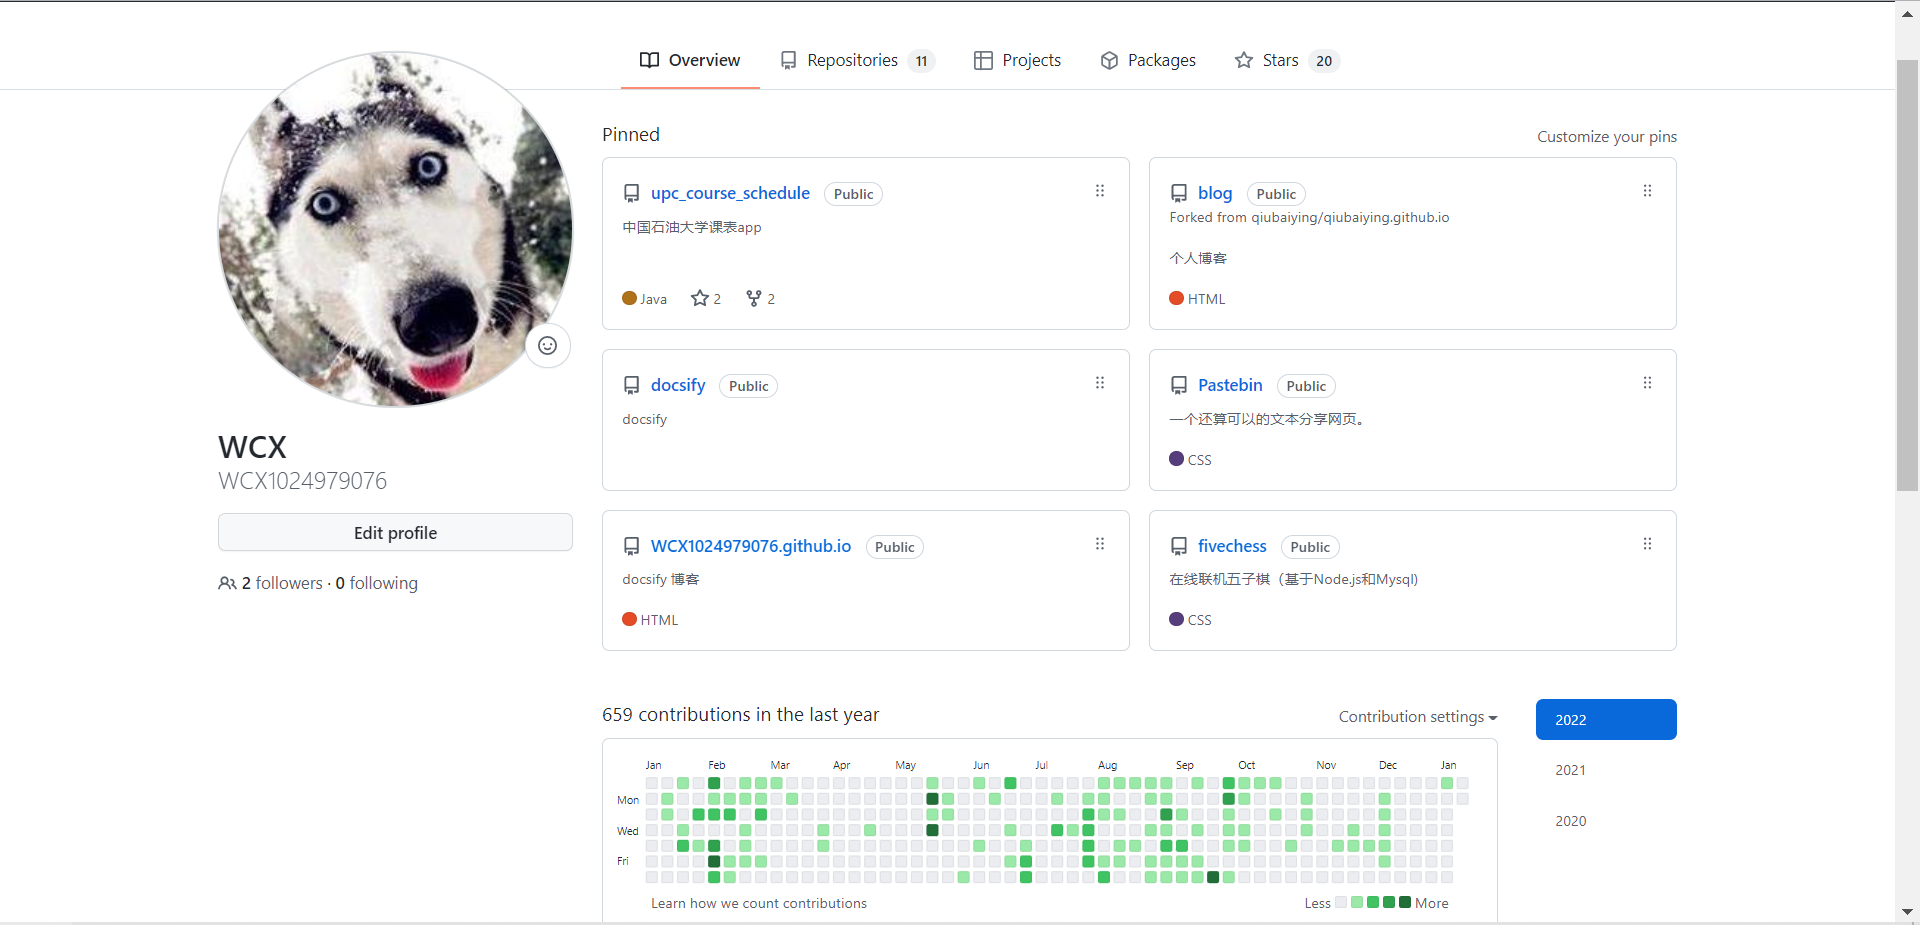
\includegraphics[width=0.95\textwidth]{github}
        \caption{Github个人网站截图}
        \label{fig:github}
        \end{figure}
        \par
        Github个人网址:https://github.com/WCX1024979076
    \item 注册观察者、学习强国、哔哩哔哩APP,给出对应的截图
        \begin{figure}[H]
        \centering
        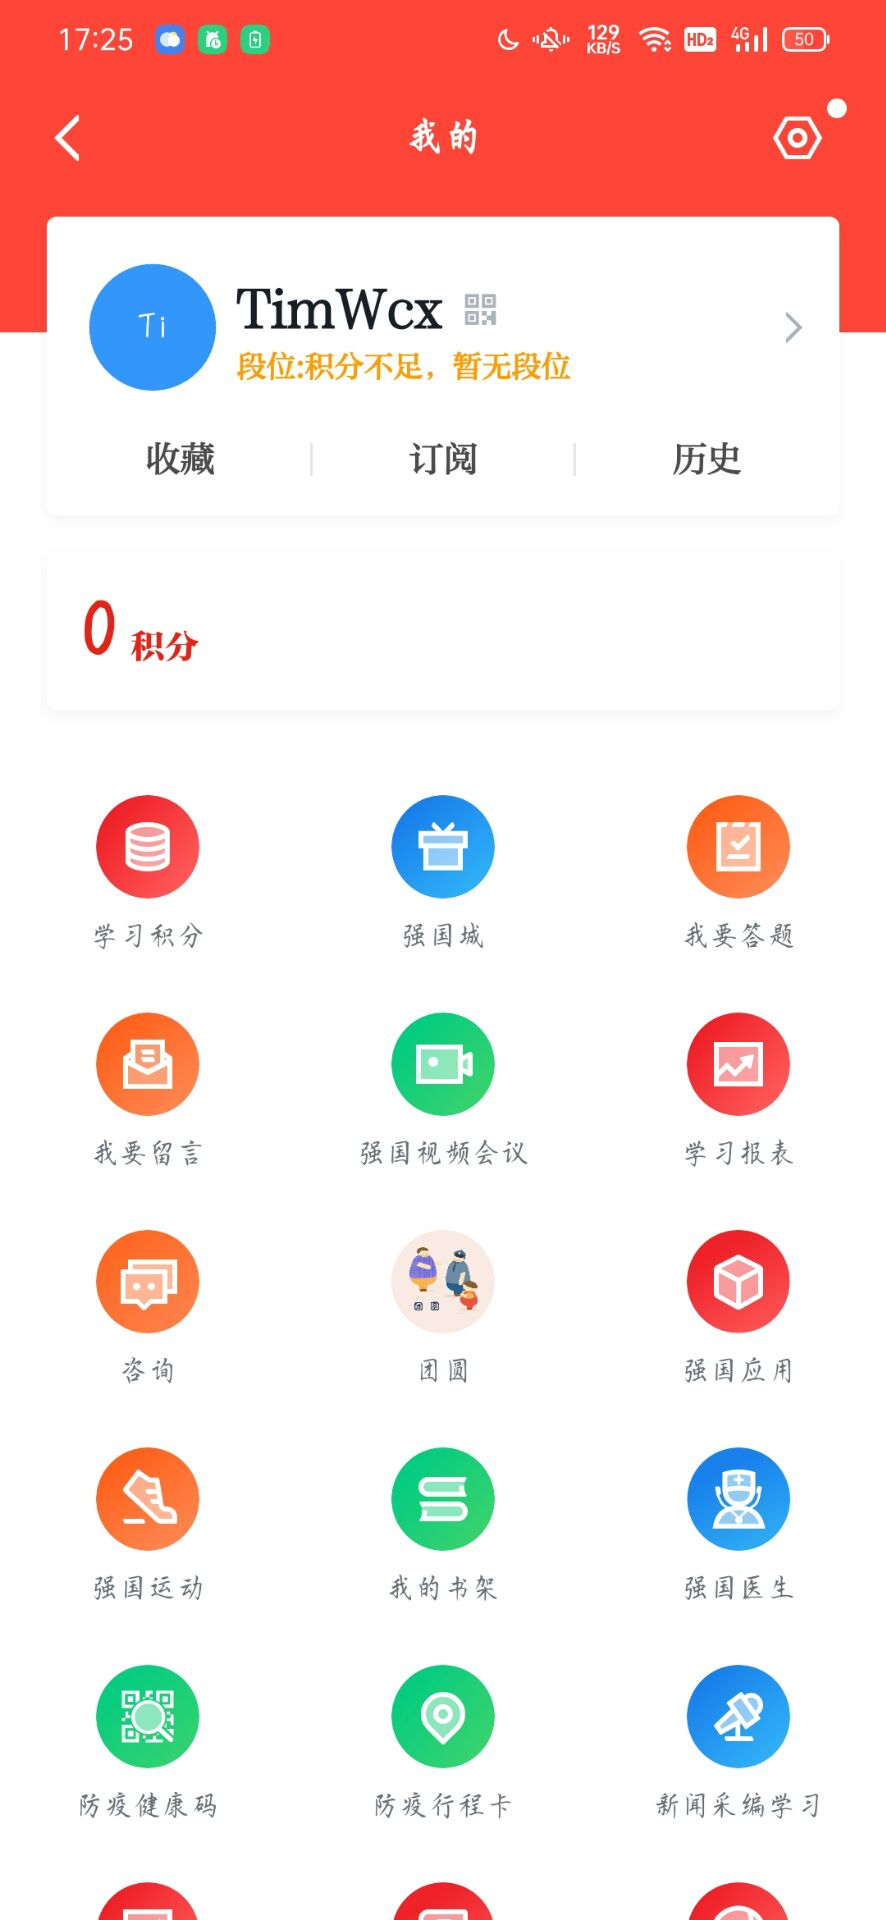
\includegraphics[width=0.4\textwidth]{xxqg.jpg}
        \hspace{1in}
        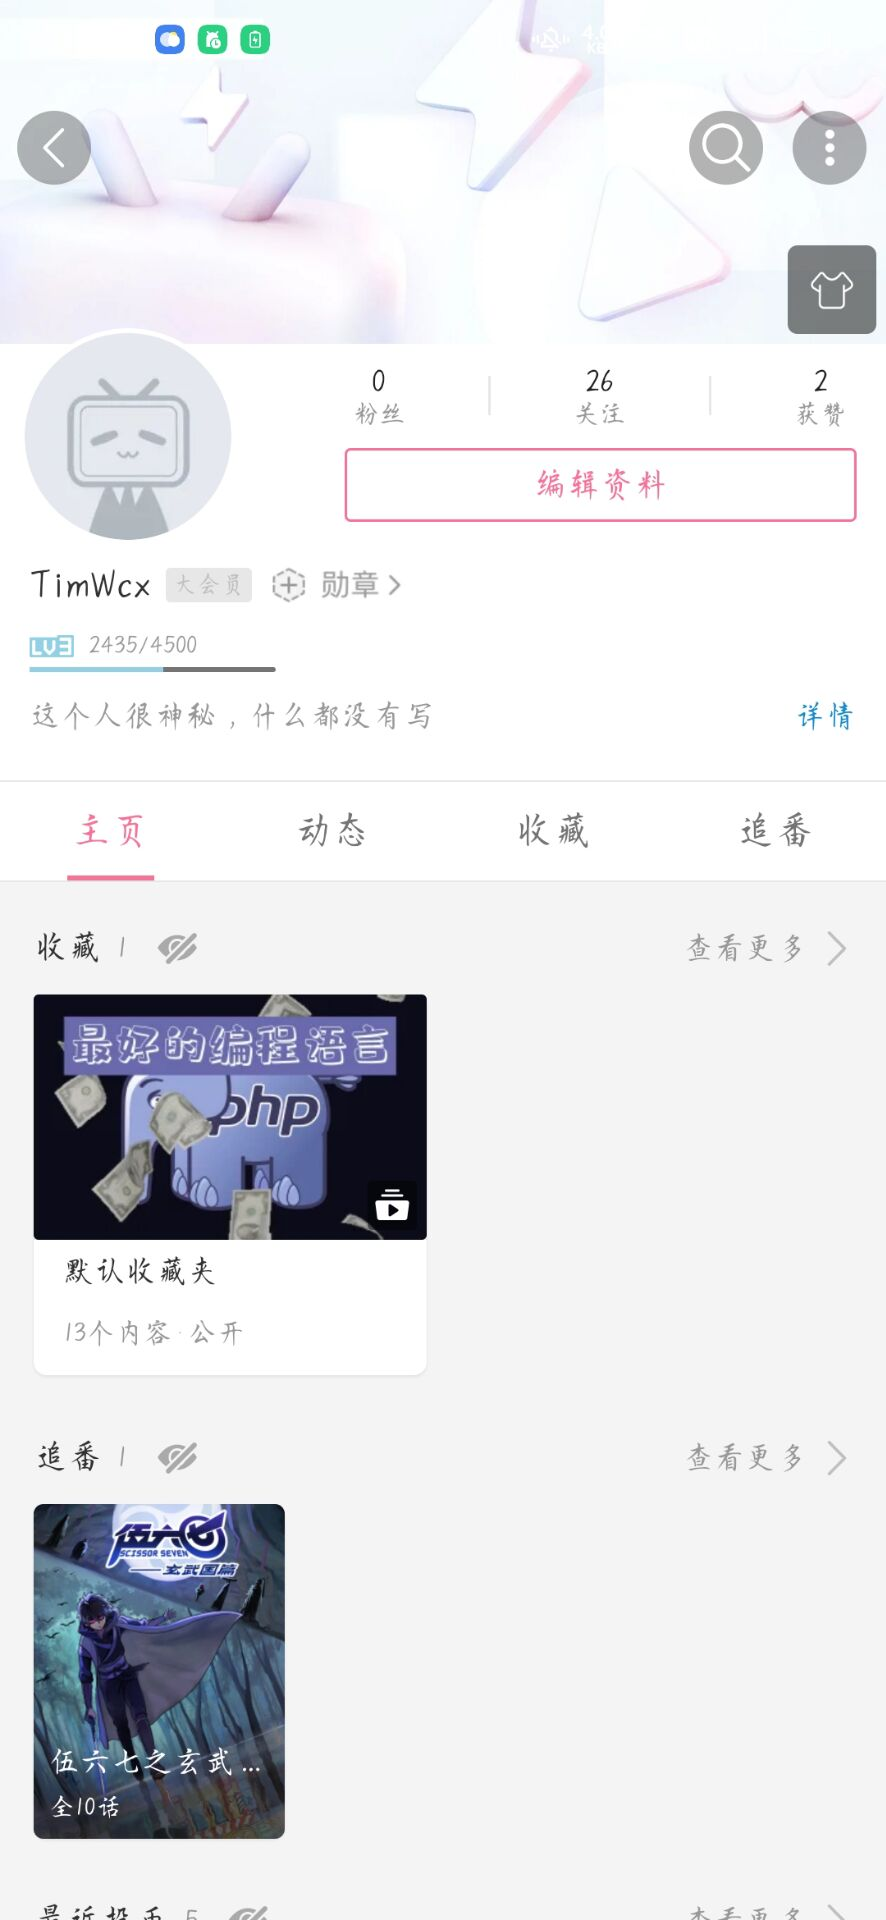
\includegraphics[width=0.4\textwidth]{bilibili.jpg}
        \caption{学习强国和哔哩哔哩APP截图}
        \end{figure}
        \begin{figure}[H]
        \centering
        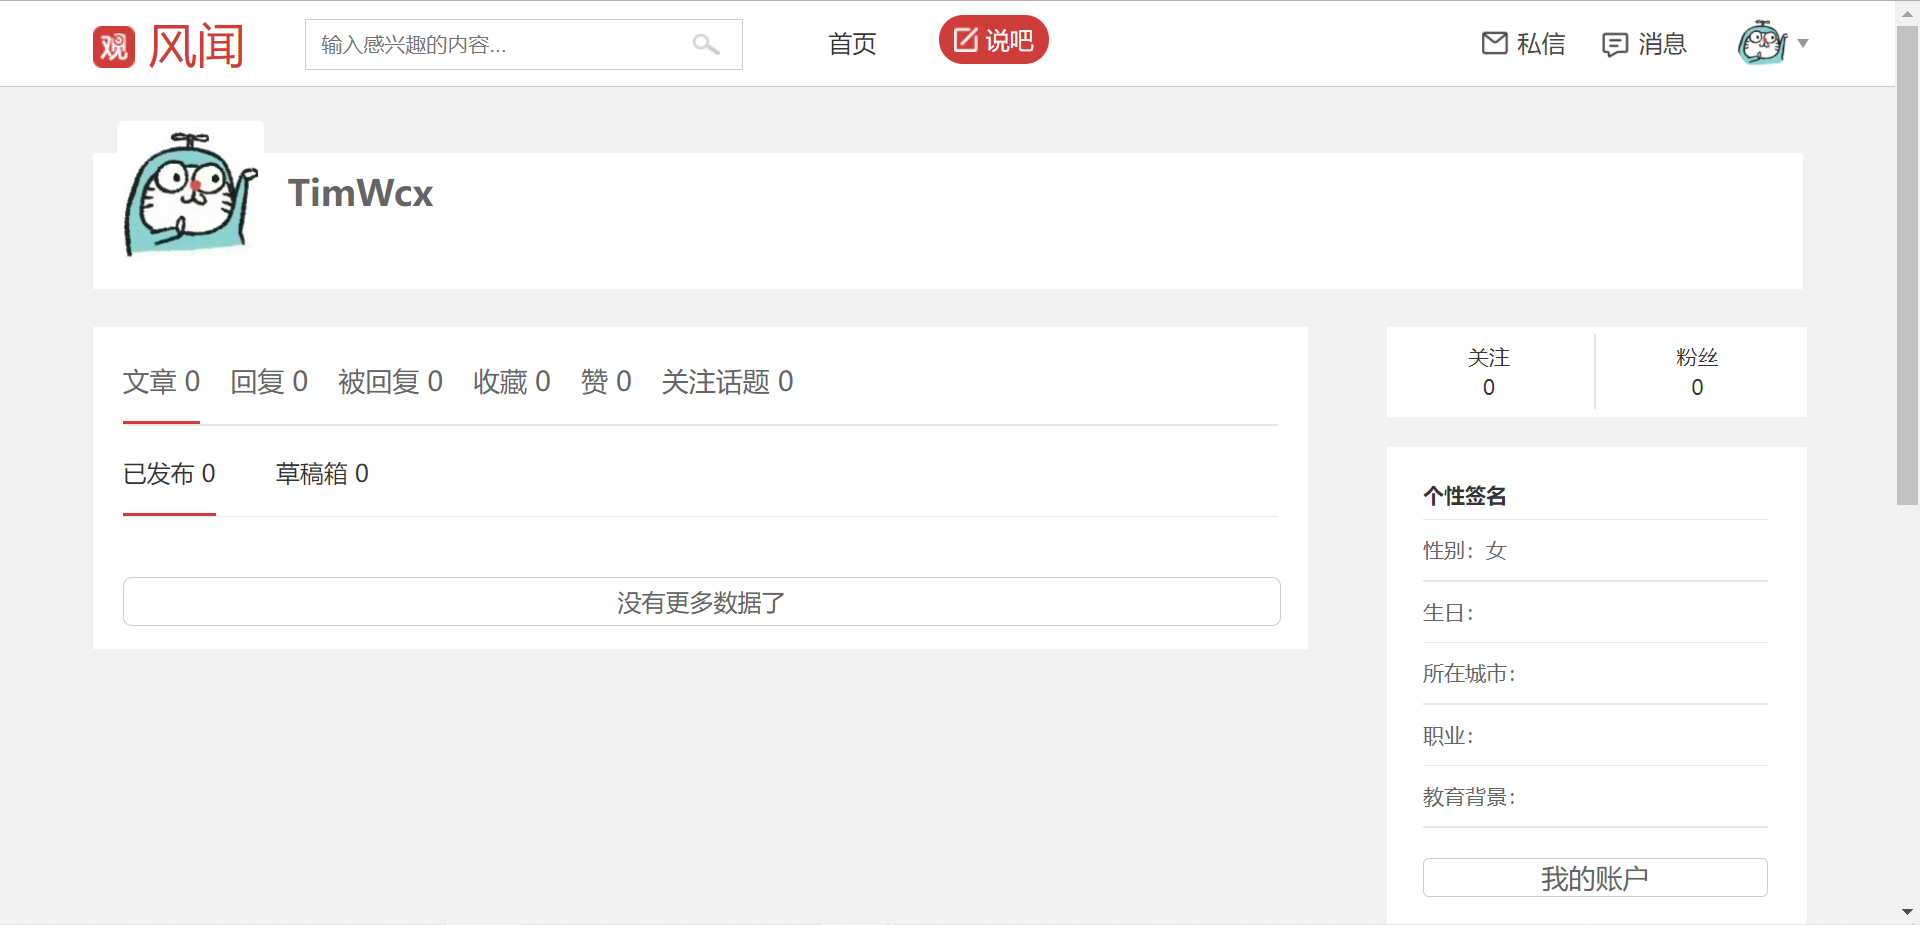
\includegraphics[width=0.95\textwidth]{guancha.png}
        \caption{观察者网站截图}
        \label{fig:guancha}
        \end{figure}

    \item 注册CSDN、博客园账户,给出个人网址和个人网站截图
        \begin{figure}[H]
        \centering
        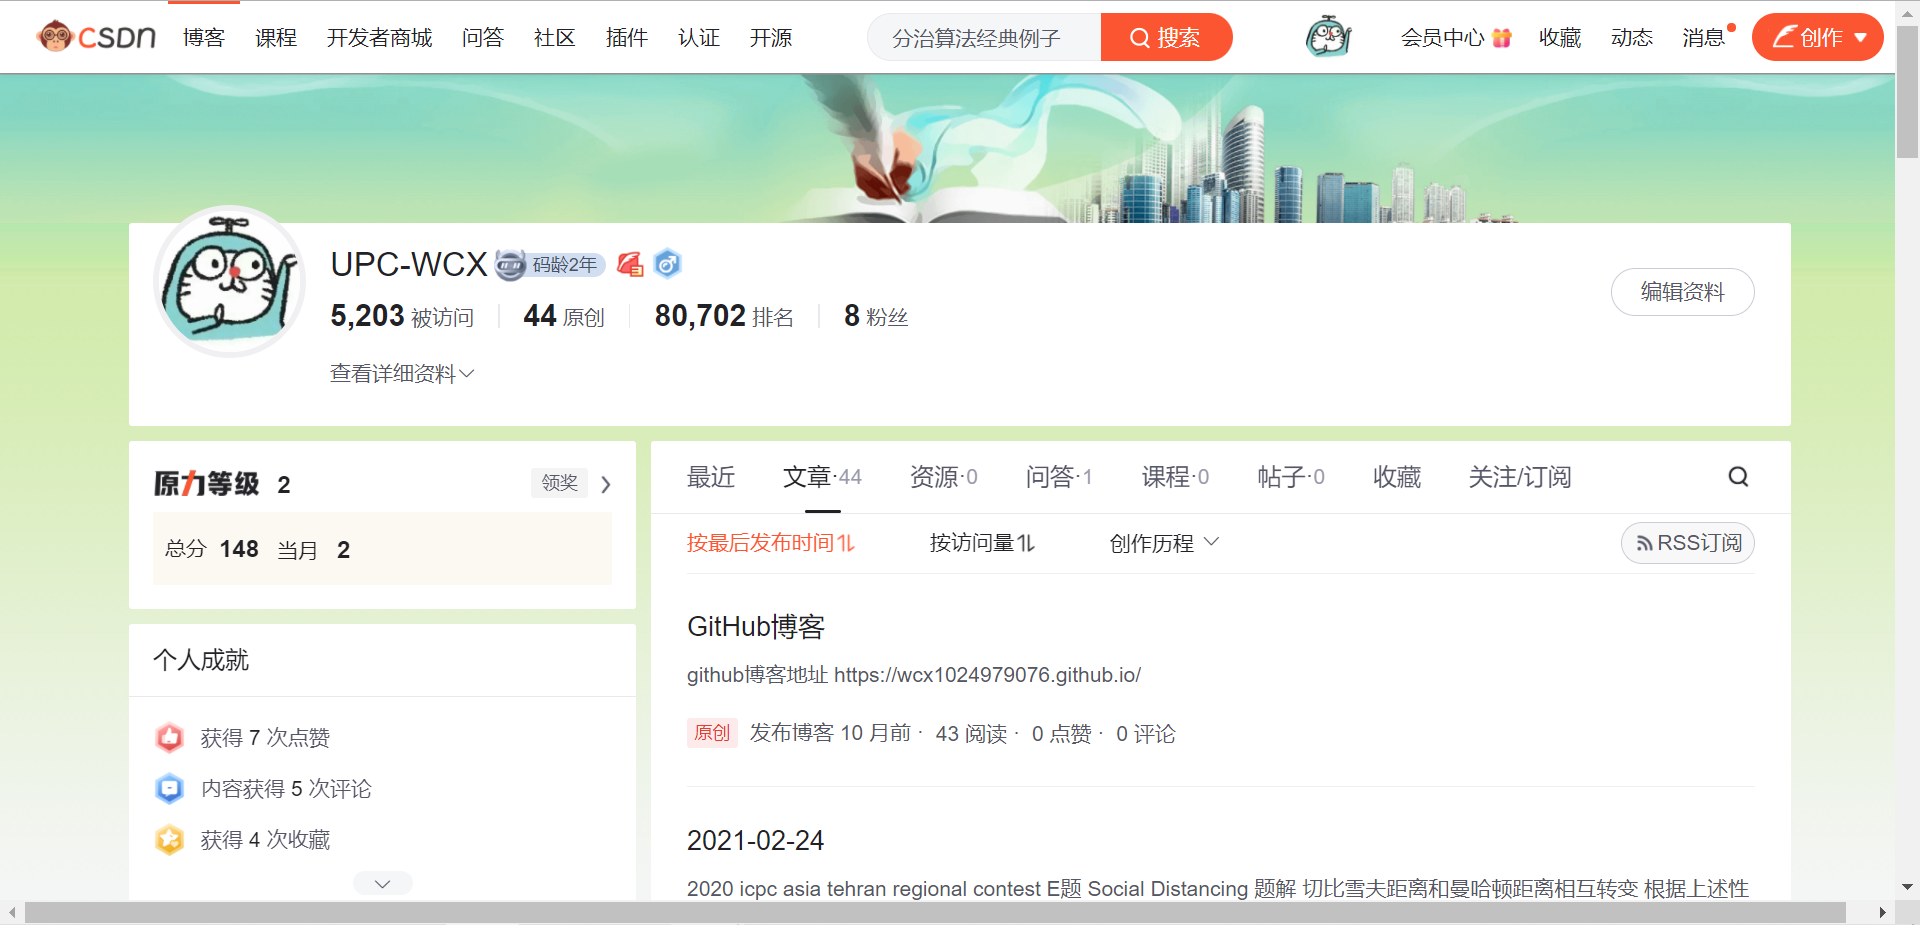
\includegraphics[width=0.95\textwidth]{csdn}
        \caption{csdn个人网站截图}
        \label{fig:csdn}
        \end{figure}
        \par
        CSDN个人网址:https://blog.csdn.net/weixin\_46048848

        \begin{figure}[H]
        \centering
        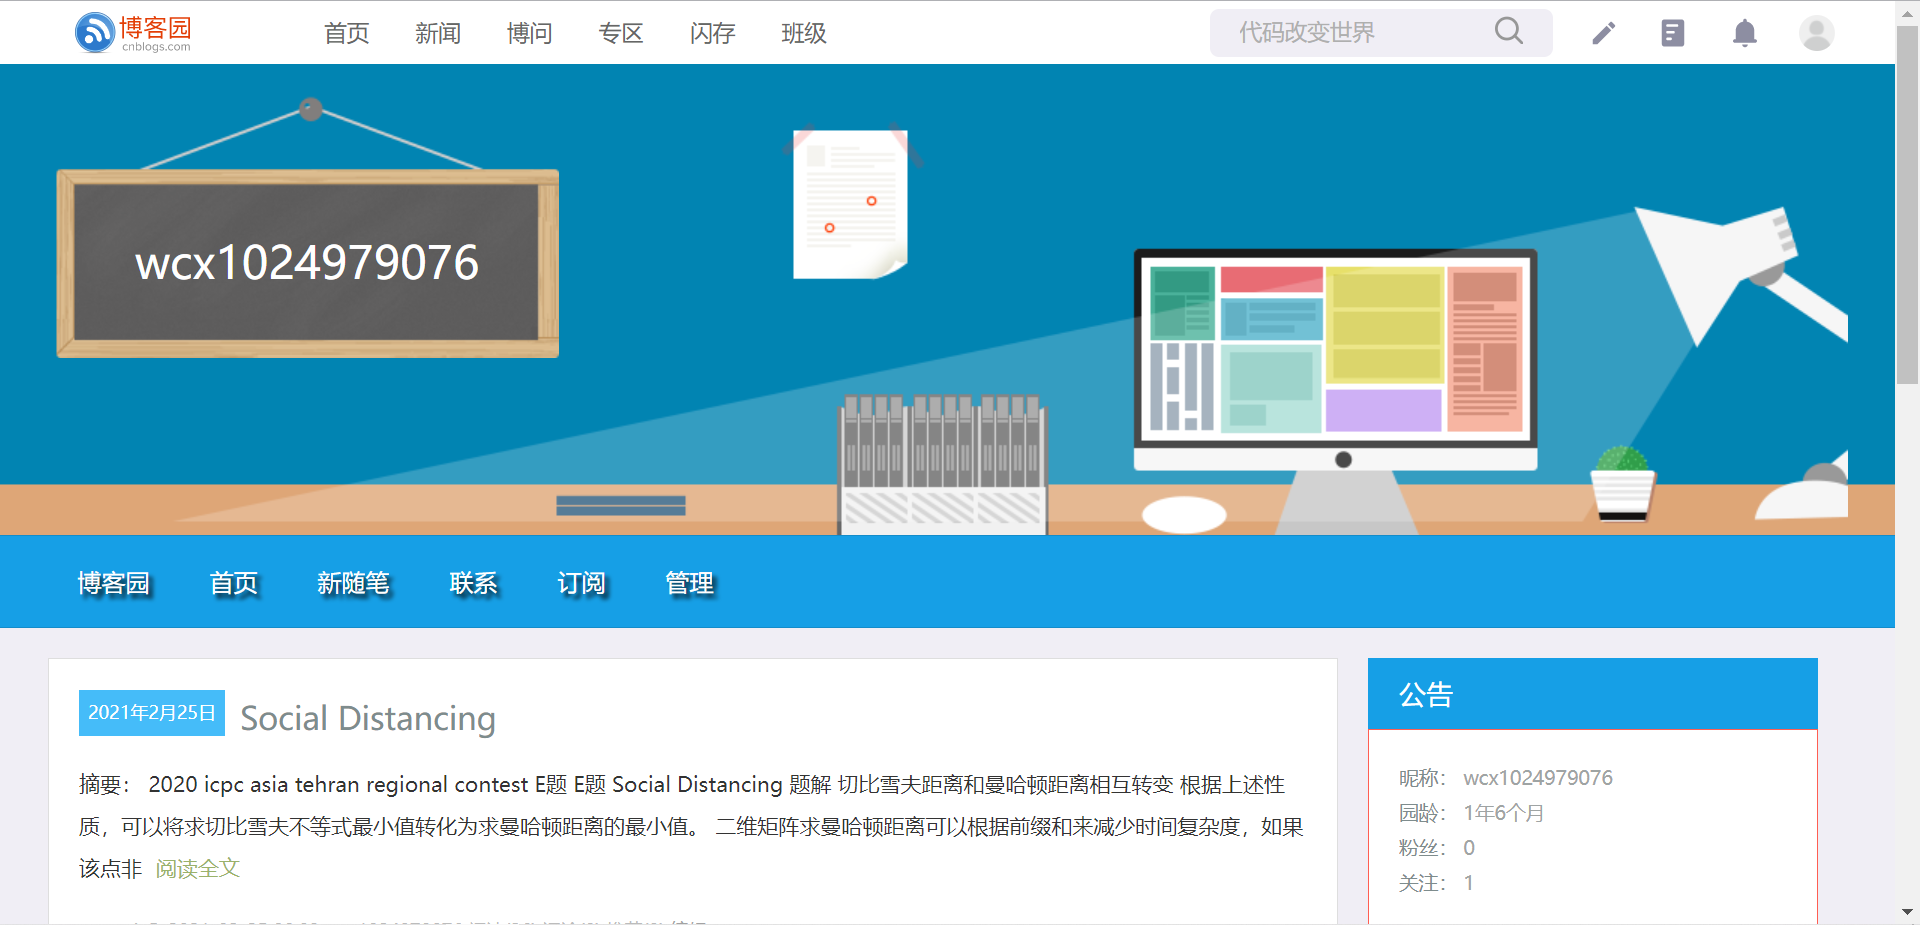
\includegraphics[width=0.95\textwidth]{cnblogs}
        \caption{博客园个人网站截图}
        \label{fig:cnblogs}
        \end{figure}
        \par
        博客园个人网址:https://www.cnblogs.com/Tim\-wcx/

    \item 注册小木虫账户,给出个人网址和个人网站截图
    
        \begin{figure}[H]
        \centering
        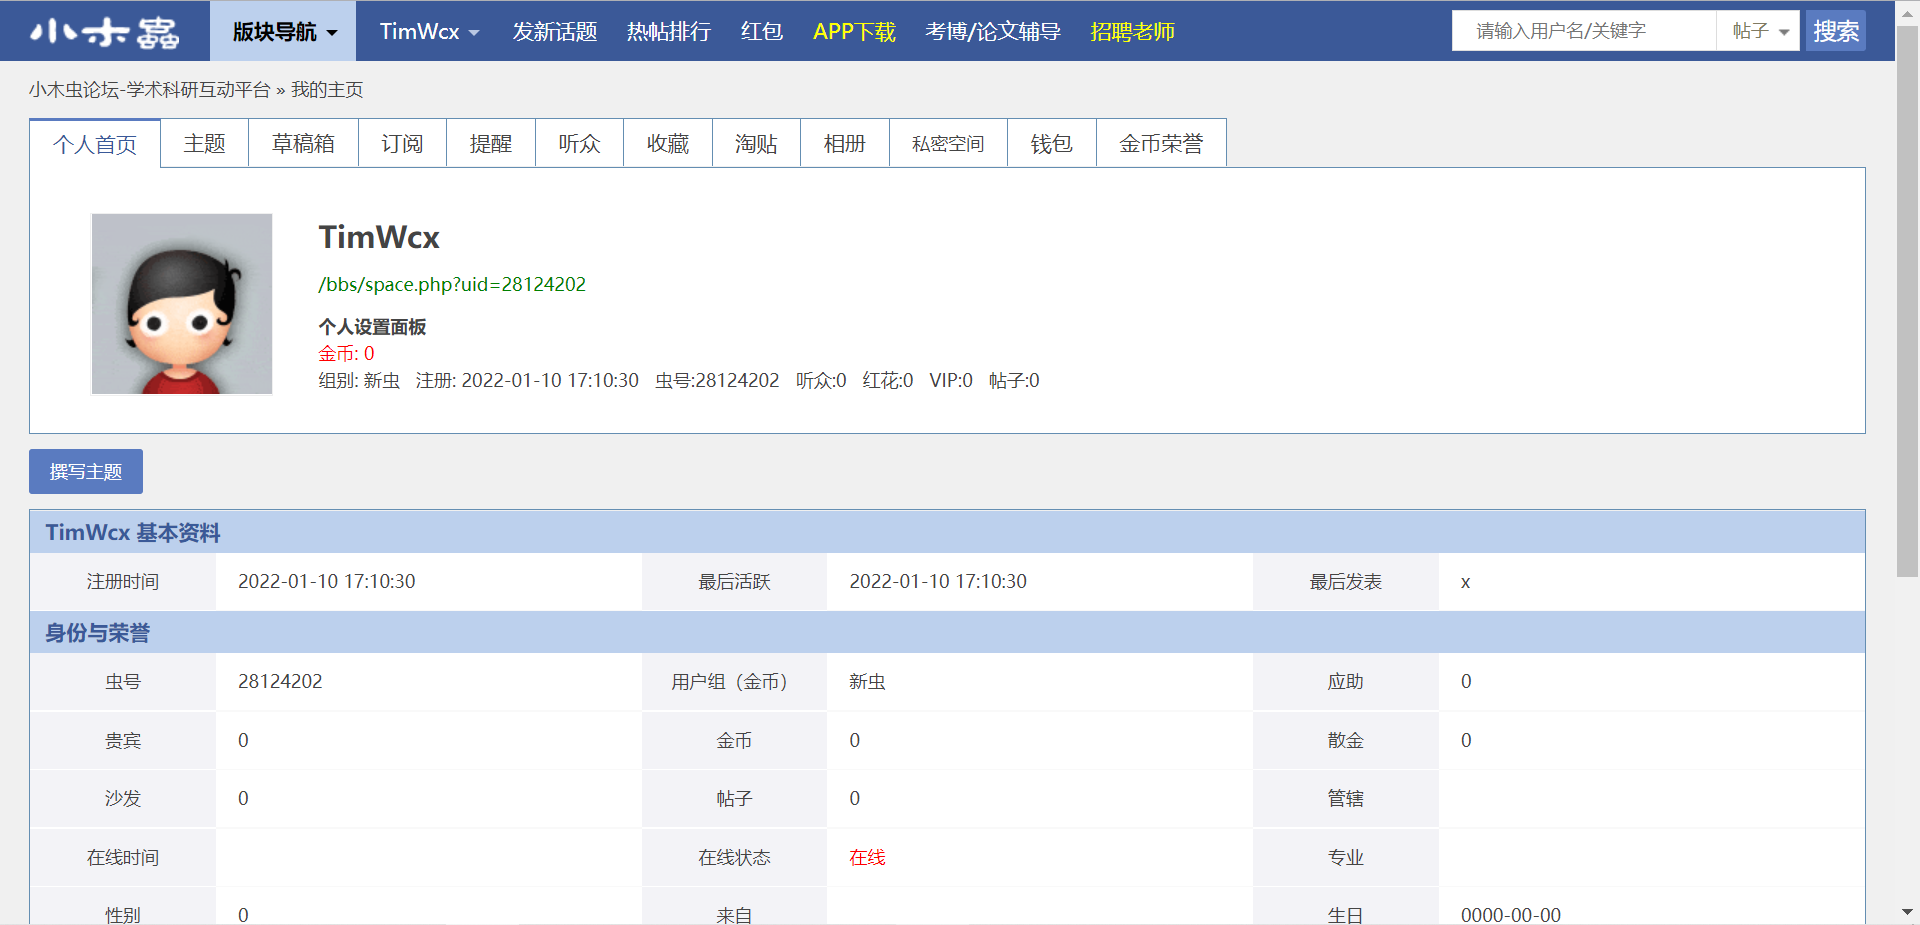
\includegraphics[width=0.95\textwidth]{muchong}
        \caption{小木虫个人网站截图}
        \label{fig:muchong}
        \end{figure}
        小木虫个人网址:http://muchong.com/bbs/space.php?uid=28124202
\end{itemize}


\hspace*{\fill} \\

{\bf 注意,参考文献至少五篇,其中至少两篇为英文文献,参考文献必须在正文中有引用。}
\bibliographystyle{plain}
\bibliography{references}


\end{document}
